\documentclass[preview]{standalone}
\usepackage{geometry}
%graphics
\usepackage{xcolor}
\usepackage{tikz}
\usetikzlibrary{shapes.geometric, shapes.multipart, arrows, calc, through,intersections}
\usepackage[caption=false,font=footnotesize]{subfig}

\tikzset{
    pics/vcell/.style = {
        code = {%
        \coordinate (-center) at (0, 0);
        \coordinate (-north) at (0, .5cm);
        \coordinate (-south) at (0,-.5cm);
        \coordinate (-east) at (.5cm,0);
        \coordinate (-west) at (-.5cm,0);
        \coordinate (-se) at (310:.5cm);
        \coordinate (-sw) at (230:.5cm);
        \coordinate (-ne) at (50:.5cm);
        \coordinate (-nw) at (130:.5cm);
        \draw[line width=2pt](0,0)circle[radius=.5cm];
        }
    },
    pics/dcell/.style = {
        code = {%
        \coordinate (-center) at (0, 0);
        \coordinate (-north) at (0, .5cm);
        \coordinate (-south) at (0,-.5cm);
        \coordinate (-east) at (.5cm,0);
        \coordinate (-west) at (-.5cm,0);
        \coordinate (-se) at (310:.5cm);
        \coordinate (-sw) at (230:.5cm);
        \coordinate (-ne) at (50:.5cm);
        \coordinate (-nw) at (130:.5cm);
        \draw[dashed,line width=2pt](0,0)circle[radius=.5cm];
        }
    },
}
\begin{document}
\begin{figure}[!t]
\centering
\subfloat[]{
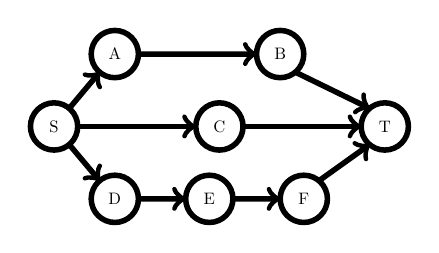
\begin{tikzpicture}[line width=2pt,transform shape, scale=0.6]
\pic(S) at (0,0){vcell};
\node at (S-center){S};

\pic(A) at (50:2){vcell};
\node at (A-center){A};
\draw[->] (S-ne) -- (A-sw);

\pic (C) at (3.5,0) {vcell};
\node at (C-center){C};
\draw[->] (S-east) -- (C-west);

\pic(D) at (310:2){vcell};
\node at (D-center){D};
\draw[->] (S-se) -- (D-nw);

\pic(B) at ($(A-east)+(3,0)$) {vcell};
\node at (B-center) {B};
\draw[->] (A-east) -- (B-west);

\pic(E) at ($(D-east)+(1.5,0)$) {vcell};
\node at (E-center) {E};
\draw[->] (D-east) -- (E-west);

\pic(F) at ($(E-east)+(1.5,0)$) {vcell};
\node at (F-center) {F};
\draw[->] (E-east) -- (F-west);

\pic(T) at (7,0) {vcell};
\node at (T-center){T};
\draw[->] (C-east) -- (T-west);
\draw[->] (B-se) -- (T-nw);
\draw[->] (F-ne) -- (T-sw);
\end{tikzpicture}
}
\subfloat[]{
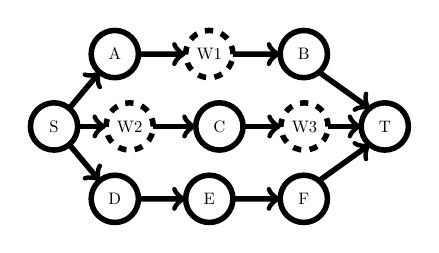
\begin{tikzpicture}[line width=2pt,transform shape, scale=0.6]
\pic(S) at (0,0){vcell};
\node at (S-center){S};

\pic(A) at (50:2){vcell};
\node at (A-center){A};
\draw[->] (S-ne) -- (A-sw);

\pic (W1) at ($(A-east)+(1.5,0)$){dcell};
\node at (W1-center) {W1};
\draw[->](A-east) -- (W1-west);

\pic(B) at ($(W1-east)+(1.5,0)$) {vcell};
\node at (B-center) {B};
\draw[->] (W1-east) -- (B-west);

\pic (W2) at ($(S-east)+(1.1,0)$){dcell};
\node at (W2-center) {W2};
\draw[->](S-east) -- (W2-west);

\pic (C) at (3.5,0) {vcell};
\node at (C-center){C};
\draw[->] (W2-east) -- (C-west);

\pic (W3) at ($(C-east)+(1.3,0)$){dcell};
\node at (W3-center) {W3};
\draw[->](C-east) -- (W3-west);

\pic(D) at (310:2){vcell};
\node at (D-center){D};
\draw[->] (S-se) -- (D-nw);

\pic(E) at ($(D-east)+(1.5,0)$) {vcell};
\node at (E-center) {E};
\draw[->] (D-east) -- (E-west);

\pic(F) at ($(E-east)+(1.5,0)$) {vcell};
\node at (F-center) {F};
\draw[->] (E-east) -- (F-west);

\pic(T) at (7,0) {vcell};
\node at (T-center){T};
\draw[->] (W3-east) -- (T-west);
\draw[->] (B-se) -- (T-nw);
\draw[->] (F-ne) -- (T-sw);
\end{tikzpicture}
}
\subfloat[]{
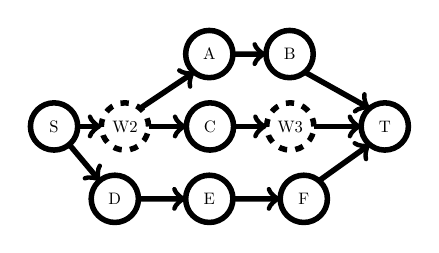
\begin{tikzpicture}[line width=2pt, transform shape, scale=0.6]
\pic(S) at (0,0){vcell};
\node at (S-center){S};

\pic(W2) at ($(S-east)+(1,0)$){dcell};
\node at (W2-center){W2};
\draw[->] (S-east) -- (W2-west);

\pic (C) at (3.3,0) {vcell};
\node at (C-center){C};
\draw[->] (W2-east) -- (C-west);

\pic(W3) at ($(C-east)+(1.2,0)$){dcell};
\node at (W3-center){W3};
\draw[->] (C-east) -- (W3-west);

\pic(A) at ($(50:2)+(2,0)$){vcell};
\node at (A-center){A};
\draw[->] (W2-ne) -- (A-sw);

\pic(B) at ($(A-east)+(1.2,0)$) {vcell};
\node at (B-center) {B};
\draw[->] (A-east) -- (B-west);

\pic(D) at (310:2){vcell};
\node at (D-center){D};
\draw[->] (S-se) -- (D-nw);

\pic(E) at ($(D-east)+(1.5,0)$) {vcell};
\node at (E-center) {E};
\draw[->] (D-east) -- (E-west);

\pic(F) at ($(E-east)+(1.5,0)$) {vcell};
\node at (F-center) {F};
\draw[->] (E-east) -- (F-west);

\pic(T) at (7,0) {vcell};
\node at (T-center){T};
\draw[->] (W3-east) -- (T-west);
\draw[->] (B-se) -- (T-nw);
\draw[->] (F-ne) -- (T-sw);
\end{tikzpicture}
}
\end{figure}
\end{document}
